\textbf{Empresa:} 10 -- AudIT\hfill\textbf{Tema:} TI-12\par
\textbf{Fecha:} 21 de septiembre de 2026

\nota{Formulario preparado conforme al punto 6 de las Indicaciones. Cada integrante completa su propio nivel de uso. La edición LaTeX documenta la asistencia de diagramación de esta sesión; no atribuye niveles ni firmas a los integrantes.}

\subsection{B.1. Declaración por sección}
\begin{center}\footnotesize\renewcommand{\arraystretch}{1.4}
\begin{tabularx}{\linewidth}{@{}p{4cm}p{1.8cm}XX@{}}
\toprule\textbf{Sección / actividad} & \textbf{Nivel} & \textbf{Herramienta y versión} & \textbf{Evidencia / estado}\\\midrule
Resumen e introducción & Por autor & Completar & Texto del maestro; confirmar declaración individual.\\
Aporte propio y análisis comparativo & Por autor & Completar & Extractos del maestro; autoría a confirmar por sus autores.\\
Marco legal e internacional & Por autor & Completar & Maestro y fuentes originales.\\
Matriz, arquitectura y economía & Por autor & Completar & Maestro y modelo de cálculo.\\
Conclusiones y recomendaciones & Por autor & Completar & Texto del maestro; confirmar declaración individual.\\
Cuestionario / presentación & Por autor & Completar & No recibidos para esta edición.\\
Diagramación LaTeX, extracción y código auxiliar & 2 & OpenCode y modelo de asistencia & Archivos fuente del informe; exportar conversación.\\\bottomrule
\end{tabularx}\end{center}
Se dispone de la declaración individual previa de Persona 1 (septiembre de 2026), con niveles 0 y 1 según actividad. Dicha declaración no representa el uso de los demás integrantes ni reemplaza la firma grupal requerida.

\subsection{B.2. Alcance de la asistencia de diagramación}
La asistencia se limitó a la extracción de contenidos del informe maestro, el ajuste de jerarquía y extensión, el formato de tablas, la rediagramación del esquema y la generación del código de compilación y verificación. El criterio sustantivo, las cifras y las fuentes corresponden al grupo; las discrepancias internas de la fuente se señalan para revisión humana en el anexo A. Las verificaciones de formato no constituyen auditoría jurídica ni acreditan cotizaciones.

\subsection{B.3. Evidencia trazable}
Fuentes de esta edición: documento principal, carpeta de extractos y scripts auxiliares de extracción y verificación, junto al informe maestro. \par
\textbf{Exportación o enlace de conversación:} \hrulefill\par
\textbf{Historial de versiones accesible al profesor:} \hrulefill

\subsection{B.4. Declaración y firma individual}
{\small Declaro que la información consignada sobre mi uso es completa y veraz; que las secciones señaladas en el punto 6.1 de las Indicaciones son de autoría humana y que puedo explicar oralmente cualquier parte del trabajo entregado.}
\begin{center}\small\renewcommand{\arraystretch}{2.4}
\begin{tabularx}{\linewidth}{@{}rXlX@{}}
\toprule\textbf{N.º} & \textbf{Nombre} & \textbf{Nivel máximo} & \textbf{Firma}\\\midrule
1 & Ignacio Cuevas & \rule{16mm}{0.2pt} & 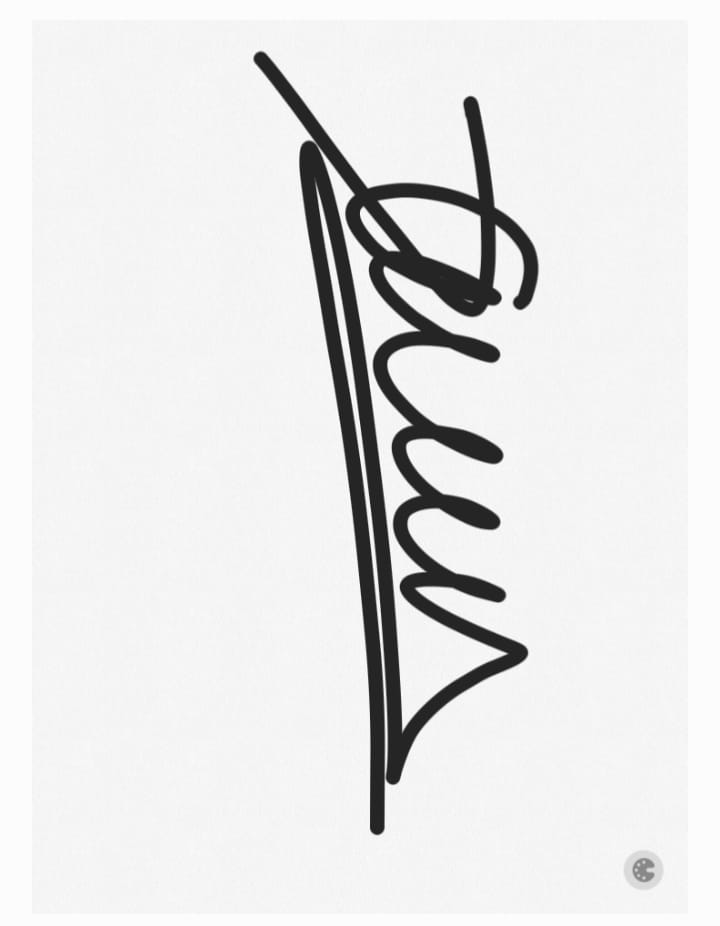
\includegraphics[height=9mm]{firmas/ignacio_cuevas.jpg}\\
2 & Alonso & \rule{16mm}{0.2pt} & 
\includegraphics[height=9mm]{firmas/alonso.jpg}\\
3 & Ignacio Vergara & \rule{16mm}{0.2pt} & 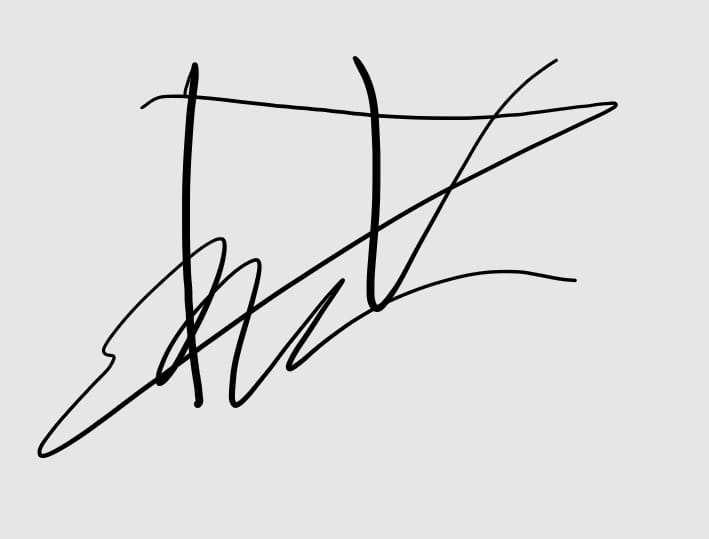
\includegraphics[height=9mm]{firmas/ignacio_v.jpg}\\
4 & Carlos Abarza & \rule{16mm}{0.2pt} & 
\includegraphics[height=9mm]{firmas/carlos.jpg}\\
5 & Martín Cevallos & \rule{16mm}{0.2pt} & 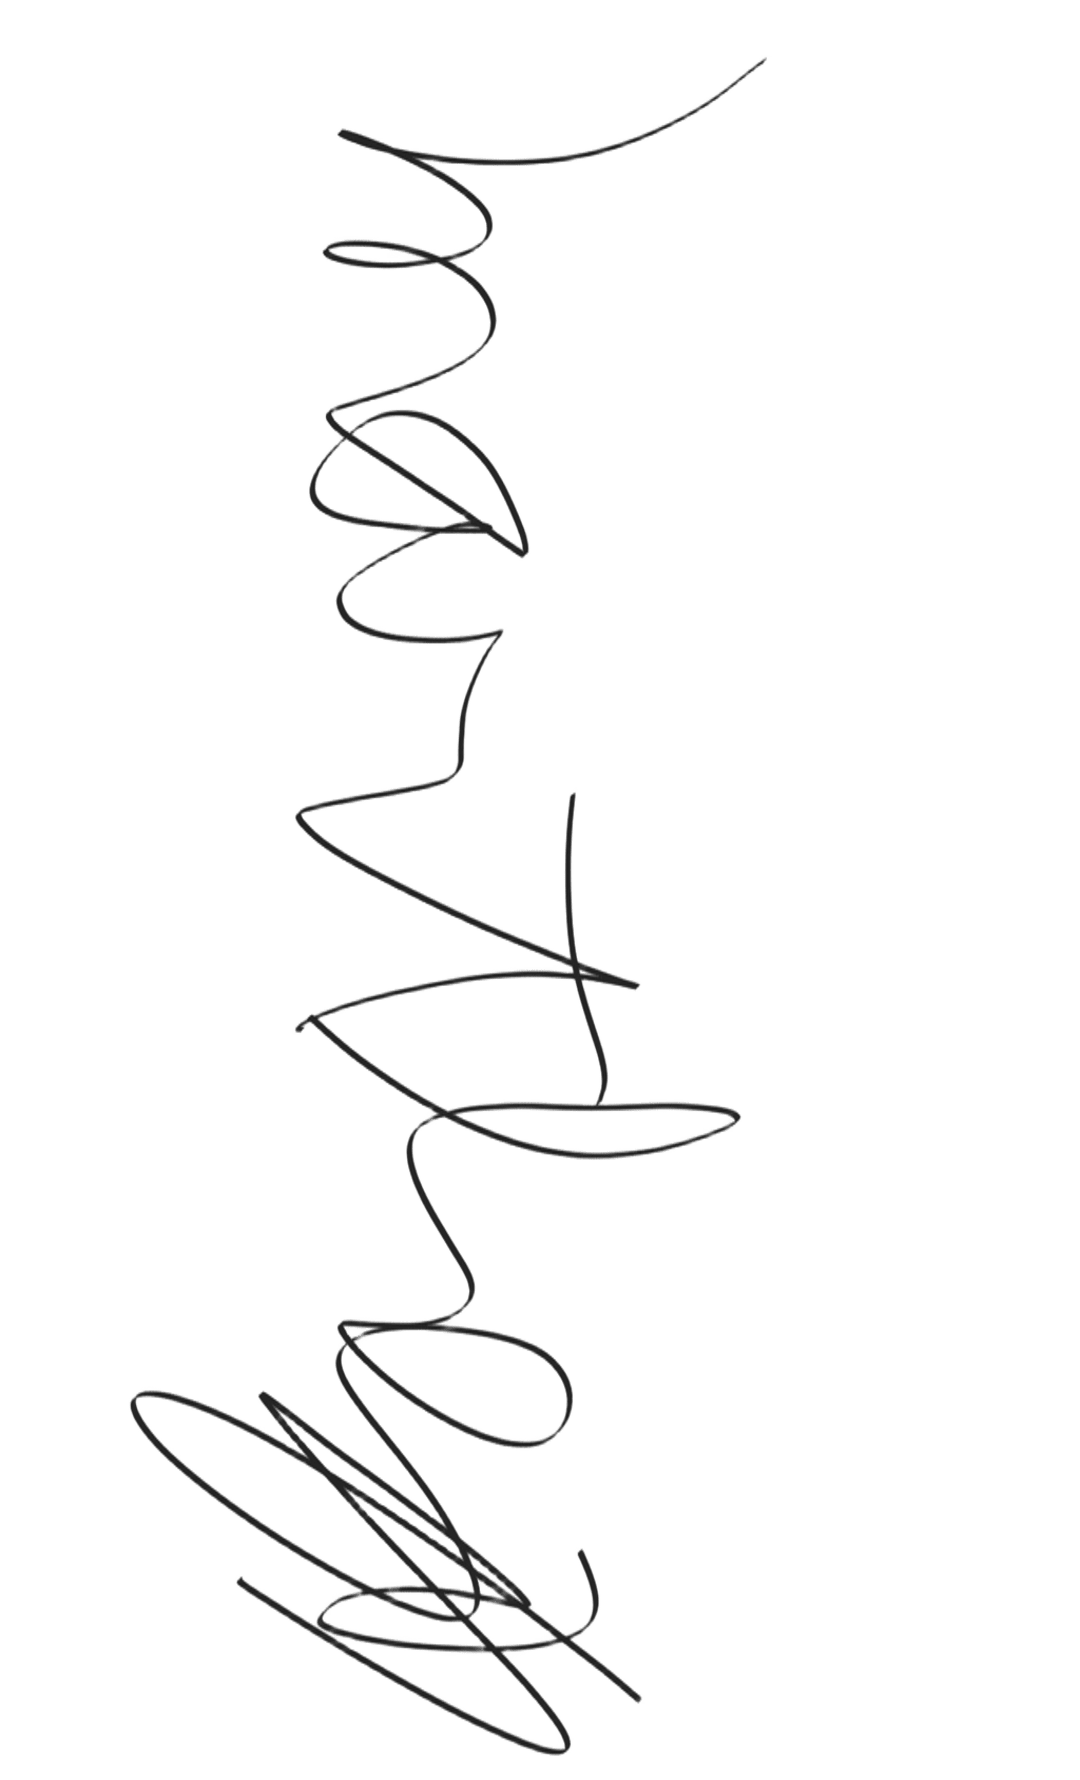
\includegraphics[height=9mm]{firmas/martin.png}\\
6 & Marcel & \rule{16mm}{0.2pt} & 
\includegraphics[height=9mm]{firmas/marcel.jpg}\\
7 & Naomi & \rule{16mm}{0.2pt} & 
\includegraphics[height=9mm]{firmas/nao.jpg}\\
8 & Matías Vergara & \rule{16mm}{0.2pt} & 
\includegraphics[height=9mm]{firmas/matias_v.jpg}\\\bottomrule
\end{tabularx}\end{center}
